\documentclass{beamer}
\usepackage{ctex, hyperref}
\usepackage[T1]{fontenc}

% other packages
\usepackage{latexsym,amsmath,xcolor,multicol,booktabs,calligra}
\usepackage{graphicx,pstricks,listings,stackengine}

\author{齐呈祥}
\title{基于 RISC-V 的 Type-1 hypervisor 的设计与实现}
\subtitle{毕业设计答辩报告}
\institute{指导老师:李罡}

\date{2023年6月6日}
\usepackage{PekingU}

\logo{
    
\includegraphics[height=0.6cm]{pic/tjulogo.png}
}

% defs
\def\cmd#1{\texttt{\color{red}\footnotesize $\backslash$#1}}
\def\env#1{\texttt{\color{blue}\footnotesize #1}}
\definecolor{deepblue}{rgb}{0,0,0.5}
\definecolor{deepred}{rgb}{0.6,0,0}
\definecolor{deepgreen}{rgb}{0,0.5,0}
\definecolor{halfgray}{gray}{0.55}

\lstset{
  basicstyle=\ttfamily\small,
  keywordstyle=\bfseries\color{deepblue},
  emphstyle=\ttfamily\color{deepred},    % Custom highlighting style
  stringstyle=\color{deepgreen},
  numbers=left,
  numberstyle=\small\color{halfgray},
  rulesepcolor=\color{red!20!green!20!blue!20},
  frame=shadowbox,
  }

  \begin{document}

  \kaishu
  \begin{frame}
    \titlepage
    % \begin{figure}[htpb]
    %   \begin{center}
    %     \includegraphics[width=1\linewidth]{./pic/TankLibBottom.png}
    %   \end{center}
    % \end{figure}
  \end{frame}

  \begin{frame}
    \addtocounter{framenumber}{-1}
    \tableofcontents[sectionstyle=show,subsectionstyle=show/shaded/hide,subsubsectionstyle=show/shaded/hide]
  \end{frame}


  \section{背景}
  \begin{frame}{Background}
    \begin{itemize} % [<+-| alert@+>] % 当然,除了alert,手动在里面插 \pause 也行
      \item 为什么需要虚拟化?
      \begin{itemize}
          \item 数据中心的数量越来越庞大,需要使用虚拟化技术实现数据中心统一管理。
          \item 物联网技术的发展,需要虚拟化技术来对物联网系统做安全保障。
      \end{itemize}
      \item 为什么要在 RISC-V ISA 上做虚拟化?
      \begin{itemize}
          \item RISC-V 目前是最流行的开源 ISA,在不到十年时间里全世界芯片出货量超过 100 亿颗。
          \item RISC-V 为国内突破卡脖子技术的关键技术,国内学术界和工业界都在积极构建基于 RISC-V 架构的产品与社区。
      \end{itemize}
    \end{itemize}
  \end{frame}

  \begin{frame}{RISC-V: the ISA}
    \begin{itemize}
        \item RISC-V 是一个开放标准 ISA
        \begin{itemize}
            \item 在 2010 年首次被伯克利开发
            \item 与商业/私有标准相区别:x86/ARM
        \end{itemize}
        \item RISC-V 传统特权级
        \begin{itemize}
            \item M(Machine)/S(Supervisor)/U(User)
        \end{itemize}
        \item RISC-V 虚拟化扩展
        \begin{itemize}
            \item 在 2021 年 11 月正式被批准
            \item S(Supervisor) -> HS(Hypervisor Supervisor)/VS(Virtual Supervisor)
        \end{itemize}
    \end{itemize}
  \end{frame}

    \begin{frame}{RISC-V: the ISA}
        \begin{columns}
            \begin{column}{0.4\textwidth}
                \centering
                \textbf{RISC-V 传统特权级}
                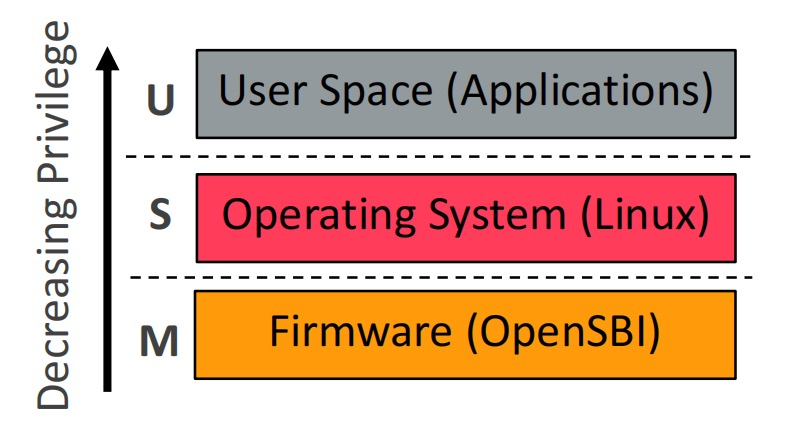
\includegraphics[width=\linewidth]{pic/tradition-priv.png}   
            \end{column}
            \begin{column}{0.6\textwidth}
                \centering
                \textbf{RISC-V Hypervisor Extension 特权级}
                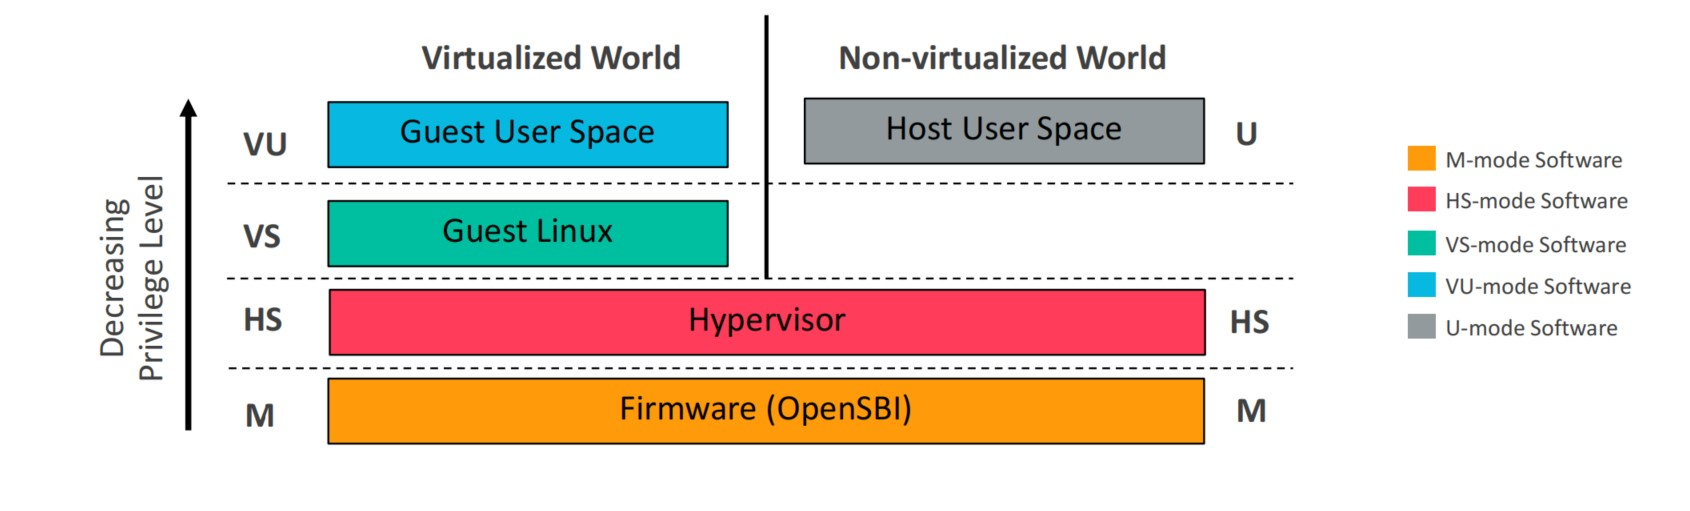
\includegraphics[width=\linewidth]{pic/h-priv.png}   
            \end{column}
        \end{columns}
    \end{frame}


  \section{设计与实现}

  \subsection{Hypocaust 设计与实现}

  \begin{frame}{Hypocaust: Design}
  
    \begin{columns}
        \begin{column}{0.5\textwidth}
            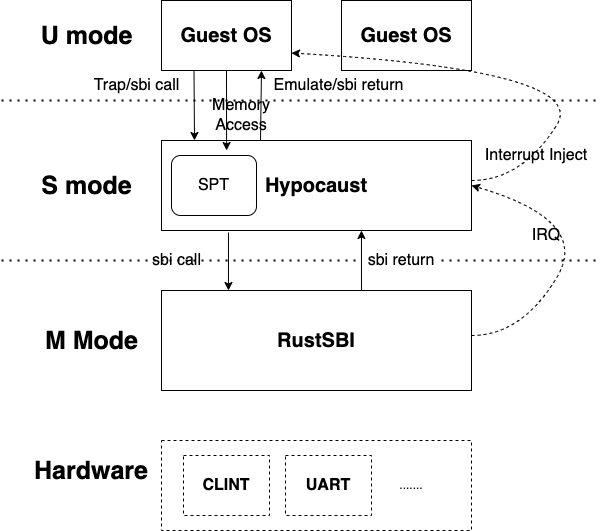
\includegraphics[width=\linewidth]{pic/hypocaust-architecture.png}          
        \end{column}
        \begin{column}{0.5\textwidth}
            \begin{itemize}
                \item CPU 虚拟化:S mode 陷入与模拟
                \item 内存虚拟化:影子页表技术
                \item 中断虚拟化:PLIC 模拟与中断转发
                \item IO 虚拟化:设备透传
                \item 系统运行:minikernel
            \end{itemize}
        \end{column}
    \end{columns}
  \end{frame}

  % \begin{frame}{Hypocaust: Pros\&Cons}
  %   \begin{itemize}
  %       \item 优势
  %       \begin{itemize}
  %           \item 可以在任何 RISC-V 平台上运行,无需支持 H Extension
  %       \end{itemize}
  %       \item 劣势
  %       \begin{itemize}
  %           \item 需要单独维护 vCPU CSR 的 Shadow State
  %           \item 维护 SPT 与 GPT 的同步关系较为复杂
  %           \item 每次读写 CSR/执行 SFENCE.VMA 指令都需要陷入处理,性能低
  %           \item 需要为每个 VM 的每个进程都维护一个影子页表,浪费内存空间
  %       \end{itemize}
  %   \end{itemize}
  % \end{frame}



  \subsection{Hypocaust-2 设计与实现}
    \begin{frame}{Hypocaust-2: Design}
  
    \begin{columns}
        \begin{column}{0.5\textwidth}
            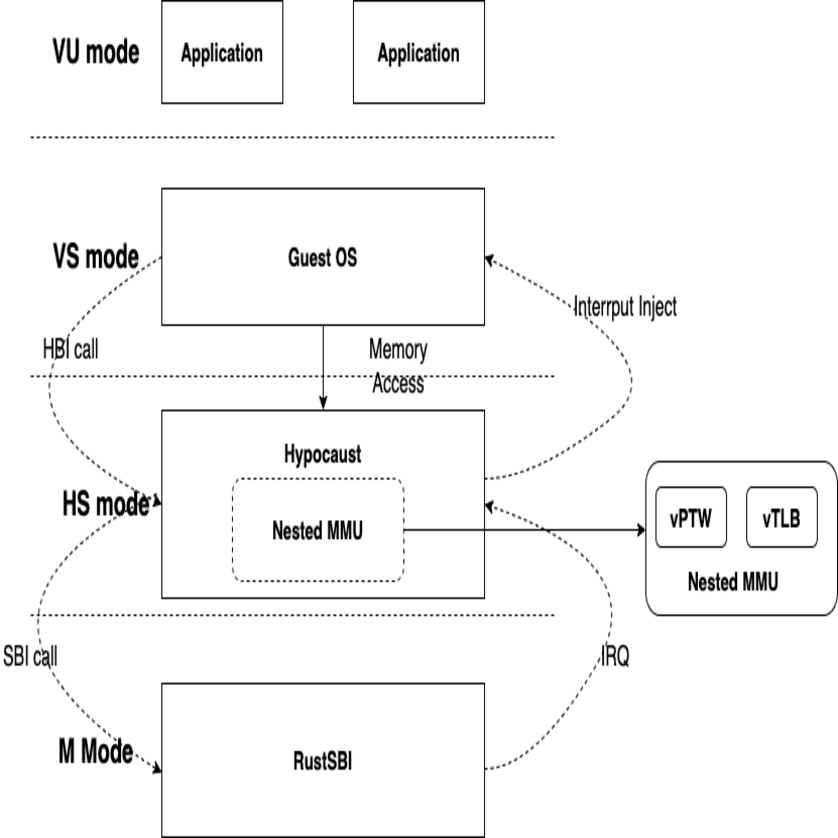
\includegraphics[width=\linewidth]{pic/hypocaust-2-arch.png}          
        \end{column}
        \begin{column}{0.5\textwidth}
            \begin{itemize}
                \item 基于设备树的配置
                \item RISC-V Hypervisor Extension 辅助虚拟化
                \item 两阶段页表翻译
                \item 异常代理与中断转发(PLIC 模拟)
                \item 设备透传
                \item 可运行 rCore-Tutorial-v3,RT-Thread 以及 Linux mainline
            \end{itemize}
        \end{column}
    \end{columns}
  \end{frame}

  % \begin{frame}{Hypocaust-2: Pros\&Cons}
  %   \begin{itemize}
  %       \item 优势
  %       \begin{itemize}
  %           \item 使用硬件辅助虚拟化技术,不需要单独为 vCPU 维护状态
  %           \item 使用 H Extension 提供的两阶段页表翻译功能,不需要维护影子页表
  %           \item 可以选择代理 VS-mode 的中断/异常,不需要每次都陷入并处理/转发中断、异常
  %           \item 实现更简单,性能更强
  %       \end{itemize}
  %       \item 劣势
  %       \begin{itemize}
  %           \item 只能在实现了 H extension 的平台上使用
  %       \end{itemize}
  %   \end{itemize}
  % \end{frame}

  \section{系统运行}

  \begin{frame}{Capable of booting system}
      \begin{columns}
          \begin{column}{0.5\textwidth}
            \centering
            \textbf{hypocaust-2 启动 RT-Thread}
            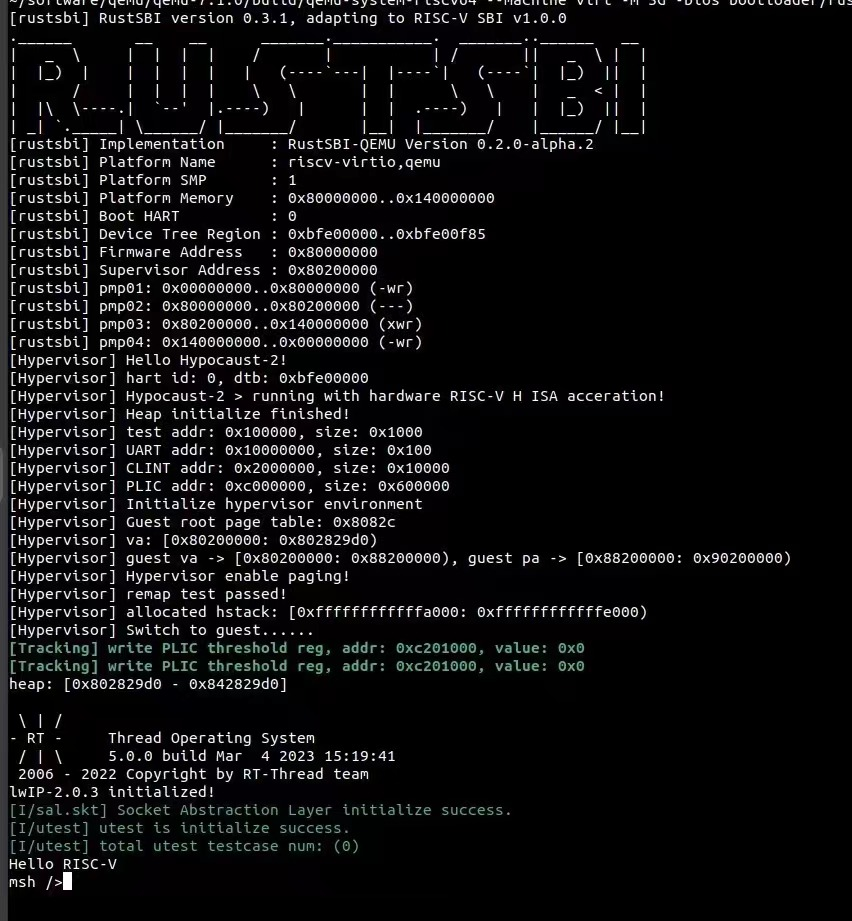
\includegraphics[width=\linewidth]{pic/hypocaust-2-rt-thread.jpeg}          
        \end{column}

        \begin{column}{0.5\textwidth}
            \centering
            \textbf{hypocaust-2 启动主线 Linux}
            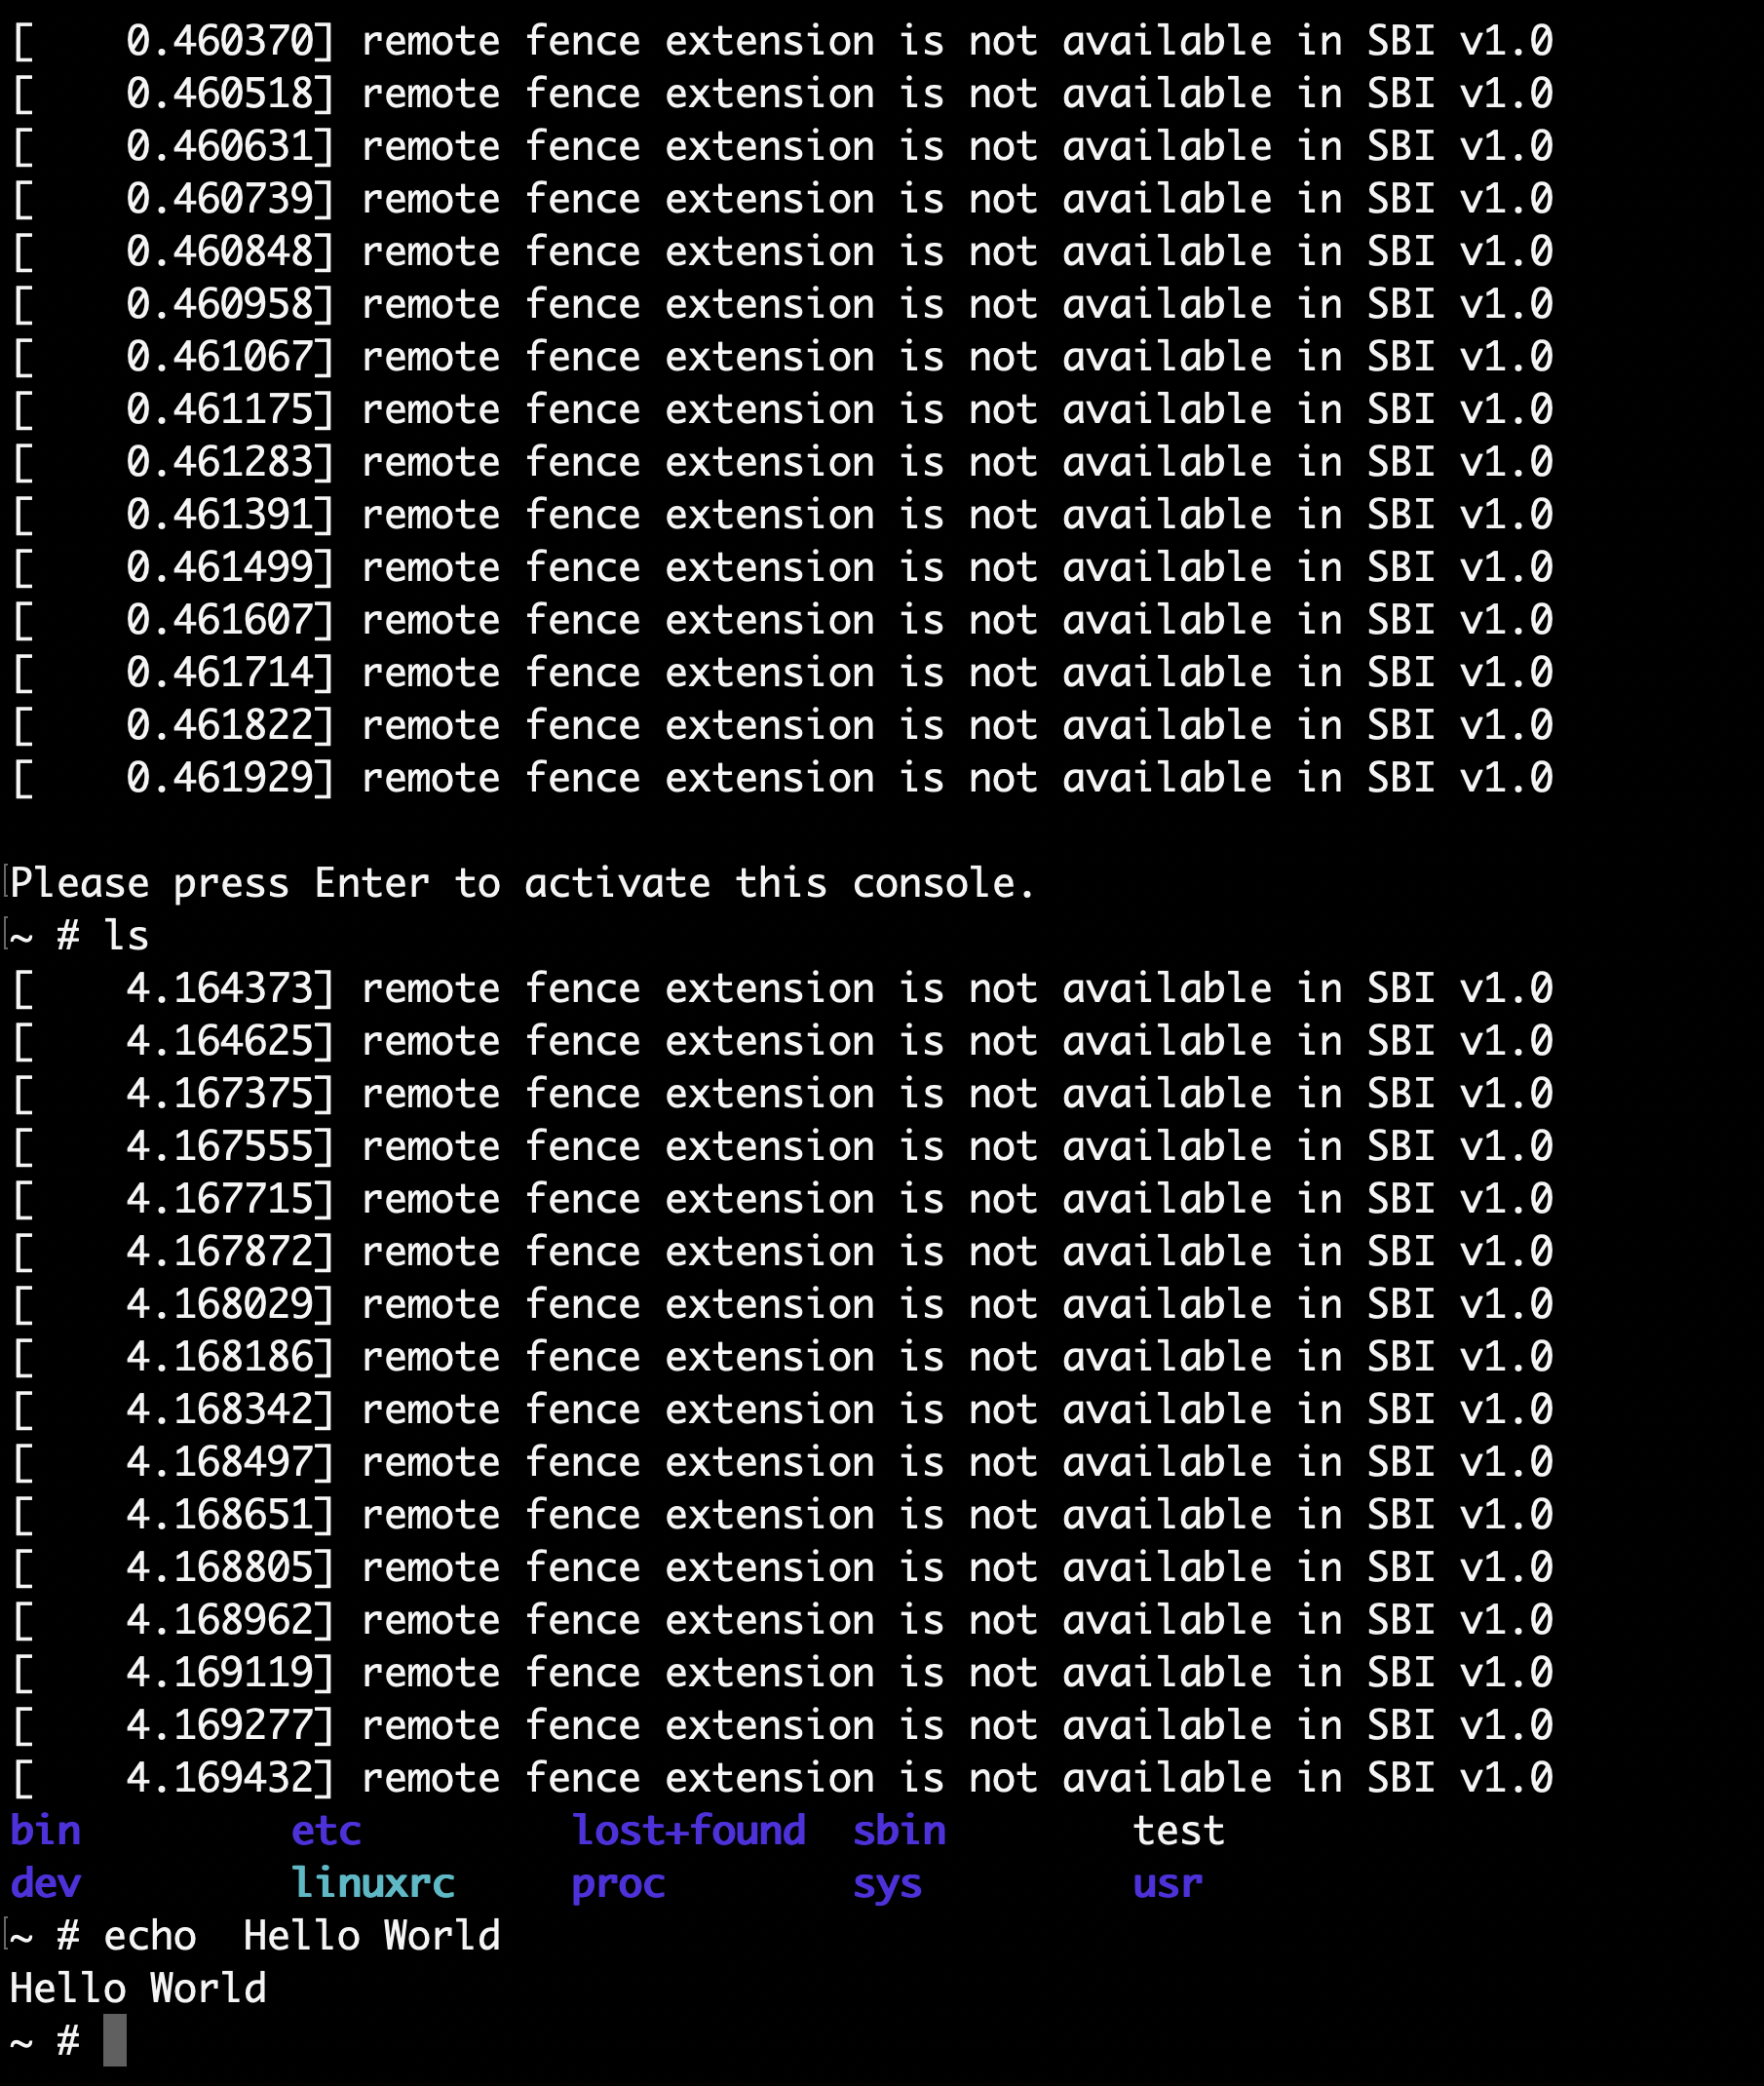
\includegraphics[width=\linewidth]{pic/hypocaust-2-linux.png}          
        \end{column}
      \end{columns}
  \end{frame}

  \section{项目进程\&展望}

  \begin{frame}{Status\&Future Works}
      \item 项目进程
      \begin{itemize}
          \item 基于 hypocaust/hypocasut-2 的经验,开发了 hypercraft(https://github.com/KuangjuX/hypercraft),一个 VMM 库,目前适配了由清华大学开发的 ArceOS 并可以类似 KVM 作为 Type-2 hypervisor 启动
          \item 搭建了一个基于 rocket-chip 带 H Extension 的软核 RISC-V SoC,并正在尝试将 hypocasut-2/hypercraft 跑在 FPGA 上。
      \end{itemize}
      \item 未来展望
      \begin{itemize}
          \item 扩展为多核/多 guest
          \item 实现 RISC-V AIA/IOMMU 驱动以提高性能和安全性
          \item 等待真实支持硬件虚拟化的 RISC-V 的芯片并移植
      \end{itemize}
  \end{frame}

  \section{Q\&A}
  \begin{frame}{Q\&A}
    \centering
    \textbf{Q\&A}
  \end{frame}

    \begin{frame}
    \centering
    \textbf{Thanks!}
  \end{frame}

\end{document}


 